\documentclass{beamer}

%\usetheme{default}
\usetheme{Boadilla}
%\usetheme{Pittsburgh}

\usecolortheme{beaver}

\setbeamercovered{transparent}
\setbeamertemplate{navigation symbols}{} %remove navigation symbols

\usepackage[english]{babel}
\usepackage[latin1]{inputenc}

\usepackage{times}
\usepackage[T1]{fontenc}

%\usepackage{animate}

% see http://tex.stackexchange.com/questions/86188/labelling-with-arrows-in-an-automated-way
\usepackage{tikz,amsmath,verbatim}

\newif\ifclipme\clipmetrue
\tikzset{labelstyle/.style={LabelStyle/.append style={#1}},linestyle/.style={LineStyle/.append style={#1}}}
\tikzset{LabelStyle/.initial={},LineStyle/.initial={}}

\newcommand{\mathWithDescription}[4][]{{%
    \tikzset{#1}%
    \tikz[baseline]{
        \node[draw=red,rounded corners,anchor=base] (m#4) {$\displaystyle#2$};
        \ifclipme\begin{pgfinterruptboundingbox}\fi
            \node[above of=m#4,font=\strut, LabelStyle] (l#4) {#3};
            \draw[-,red, LineStyle] (l#4) to (m#4);
        \ifclipme\end{pgfinterruptboundingbox}\fi
    }%
}}

\newcommand{\mathWithDescriptionStarred}[3][]{{%
    \clipmefalse%
    \mathWithDescription[#1]{#2}{#3}{\themathLabelNode}%
}}

\newcounter{mathLabelNode}

\newcommand{\mathLabelBox}[3][]{%
   \stepcounter{mathLabelNode}%
   \mathWithDescription[#1]{#2}{#3}{\themathLabelNode}%
   \vphantom{\mathWithDescriptionStarred[#1]{#2}{#3}{\themathLabelNode}}%
}

% math macros
\newcommand\bb{\mathbf{b}}
\newcommand\bbf{\mathbf{f}}
\newcommand\bn{\mathbf{n}}
\newcommand\bq{\mathbf{q}}
\newcommand\bu{\mathbf{u}}
\newcommand\bv{\mathbf{v}}
\newcommand\bx{\mathbf{x}}
\newcommand\by{\mathbf{y}}

\newcommand\bF{\mathbf{F}}
\newcommand\bQ{\mathbf{Q}}
\newcommand\bV{\mathbf{V}}
\newcommand\bX{\mathbf{X}}

\newcommand\CC{\mathbb{C}}
\newcommand\RR{\mathbb{R}}

\newcommand{\DDt}[1]{\ensuremath{\frac{d #1}{d t}}}
\newcommand{\ddt}[1]{\ensuremath{\frac{\partial #1}{\partial t}}}

\newcommand\Div{\nabla\cdot}
\newcommand\eps{\epsilon}
\newcommand\grad{\nabla}
\newcommand{\ip}[2]{\ensuremath{\left<#1,#2\right>}}
\newcommand\nhat{\mathbf{n}}
\newcommand\lam{\lambda}
\newcommand\lap{\triangle}
\newcommand\Matlab{\textsc{Matlab}\xspace}
\newcommand\vf{\varphi}


\title[Computing glacier geometry]{Computing glacier geometry \\ in nonlinear complementarity problem form}

\author{Ed Bueler}

\institute[UAF] % (optional, but mostly needed)
{
  Dept of Mathematics and Statistics, and Geophysical Institute\\
  University of Alaska Fairbanks \\
  \tiny (\emph{funded by NASA Modeling, Analysis, and Prediction program})%
}

\date[Copper Mtn 2016]{Copper Mountain Iterative March 2016}


\begin{document}
\graphicspath{{../../talks-public/commonfigs/}}

\begin{frame}
  \titlepage
\end{frame}


\begin{frame}{outline}
  \tableofcontents
\end{frame}


\section{NCPs and VIs}

\begin{frame}{nonlinear complementarity problems (NCP)}

\begin{itemize}
\item abstractly, NCP is:
  \begin{itemize}
  \item[$\circ$]  given differentiable map $\bF:\RR^n \to \RR^n$
  \item[$\circ$]  solve for $\bx\in\RR^n$:
     $$\bx \ge 0, \quad \bF(\bx) \ge 0, \quad \bx^\top \bF(\bx) = 0$$
  \end{itemize}
\item toy problem:  FIXME show 1D obstacle
\item our case:
  \begin{itemize}
  \item[$\circ$]  $\infty$ dimensions
  \item[$\circ$] comes from with mass conservation (MC) equation $H_t + \Div\bq = f$
  \item[$\circ$]  $\bx = H$ and $\bF(\bx) = (\text{residual from discrete-time  MC eqn.})$
  \end{itemize}
\end{itemize}
\end{frame}


\begin{frame}{variational inequalities (VI)}

\begin{itemize}
\item abstractly, in finite dimensions, VI is:
  \begin{itemize}
  \item[$\circ$]  given differentiable map $\bF:\RR^n \to \RR^n$
  \item[$\circ$]  solve for $\bx\in\RR^n$:
     $$\ip{\bF(\bx)}{\by-\bx} \ge 0 \quad \forall \by \in \mathcal{K}$$
  \end{itemize}
\item toy problem:  FIXME show 1D obstacle
\item in finite dimensions: VI $\leftrightarrow$ NCP
\end{itemize}
\end{frame}


\begin{frame}{these problems are \emph{intrinsically nonlinear}}

\begin{itemize}
\item even if $\bF(\bx)$ is linear, problem is nonlinear
  \begin{itemize}
  \item[$\circ$]  solution space is not affine
  \end{itemize}
\item toy problem:  FIXME show 1D obstacle
\item iteration appropriate
  \begin{itemize}
  \item[$\circ$]  in infinite dimensions, iteration is obligatory
  \end{itemize}
\end{itemize}
\end{frame}


\begin{frame}{these glacier problems are \emph{not} optimizations}

\begin{itemize}
\item NCP and VI problems arising in glacier problems are not (generally) constrained optimization problems
  \begin{itemize}
  \item[$\circ$]  no surprise: the mass continuity equation is not (generally) an Euler-Lagrange (variational) equation of a functional
  \item[$\circ$]  Jouvet \& Bueler (2012) solve problem as fixed-point sequence of optimizations, but this loses Newton quadratic convergence character
  \end{itemize}
\item Jacobians are \emph{not} generally symmetric
\end{itemize}
\end{frame}


\AtBeginSection[] % Do nothing for \section*
{
\begin{frame}<beamer>
\frametitle{outline}
\tableofcontents[currentsection]
\end{frame}
}

\section{glacier geometry-evolution models}

\begin{frame}{coupled mass and momentum equations}

\begin{itemize}
\item FIXME
\end{itemize}
\end{frame}


\begin{frame}{a free-boundary fluid layer in a climate}

\begin{center}
\includegraphics[width=0.95\textwidth,keepaspectratio=true]{cartoon-wclimate}
\end{center}

\vspace{-7mm}
  \begin{itemize}
  \item mass conservation PDE for a layer:
      $$h_t + \Div\bq = {\color{blue} f}$$
    \begin{itemize}
    \vspace{-4mm}
    \item[$\circ$] $h$ is a thickness: $h\ge 0$
    \item[$\circ$] mass conservation PDE applies only where $h>0$
    \item[$\circ$] $\bq$ is flow (vertically-integrated)
    \item[$\circ$] source ${\color{blue} f}$ is ``climate''; ${\color{blue} f}>0$ shown downward
    \end{itemize}
  \end{itemize}
\end{frame}


\begin{frame}{examples with similar character}

\includegraphics[width=0.4\textwidth,keepaspectratio=true]{polaris}
\hfill
\includegraphics[width=0.45\textwidth,keepaspectratio=true]{supp4rignot-small}

\small glaciers \hfill ice shelves \& sea ice

\medskip
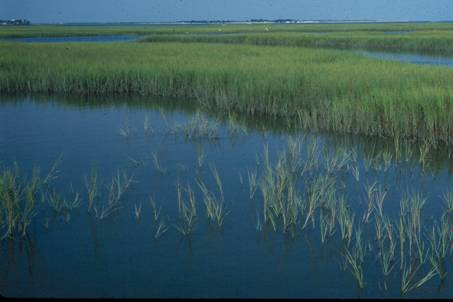
\includegraphics[width=0.41\textwidth,keepaspectratio=true]{marsh-water}
\hfill
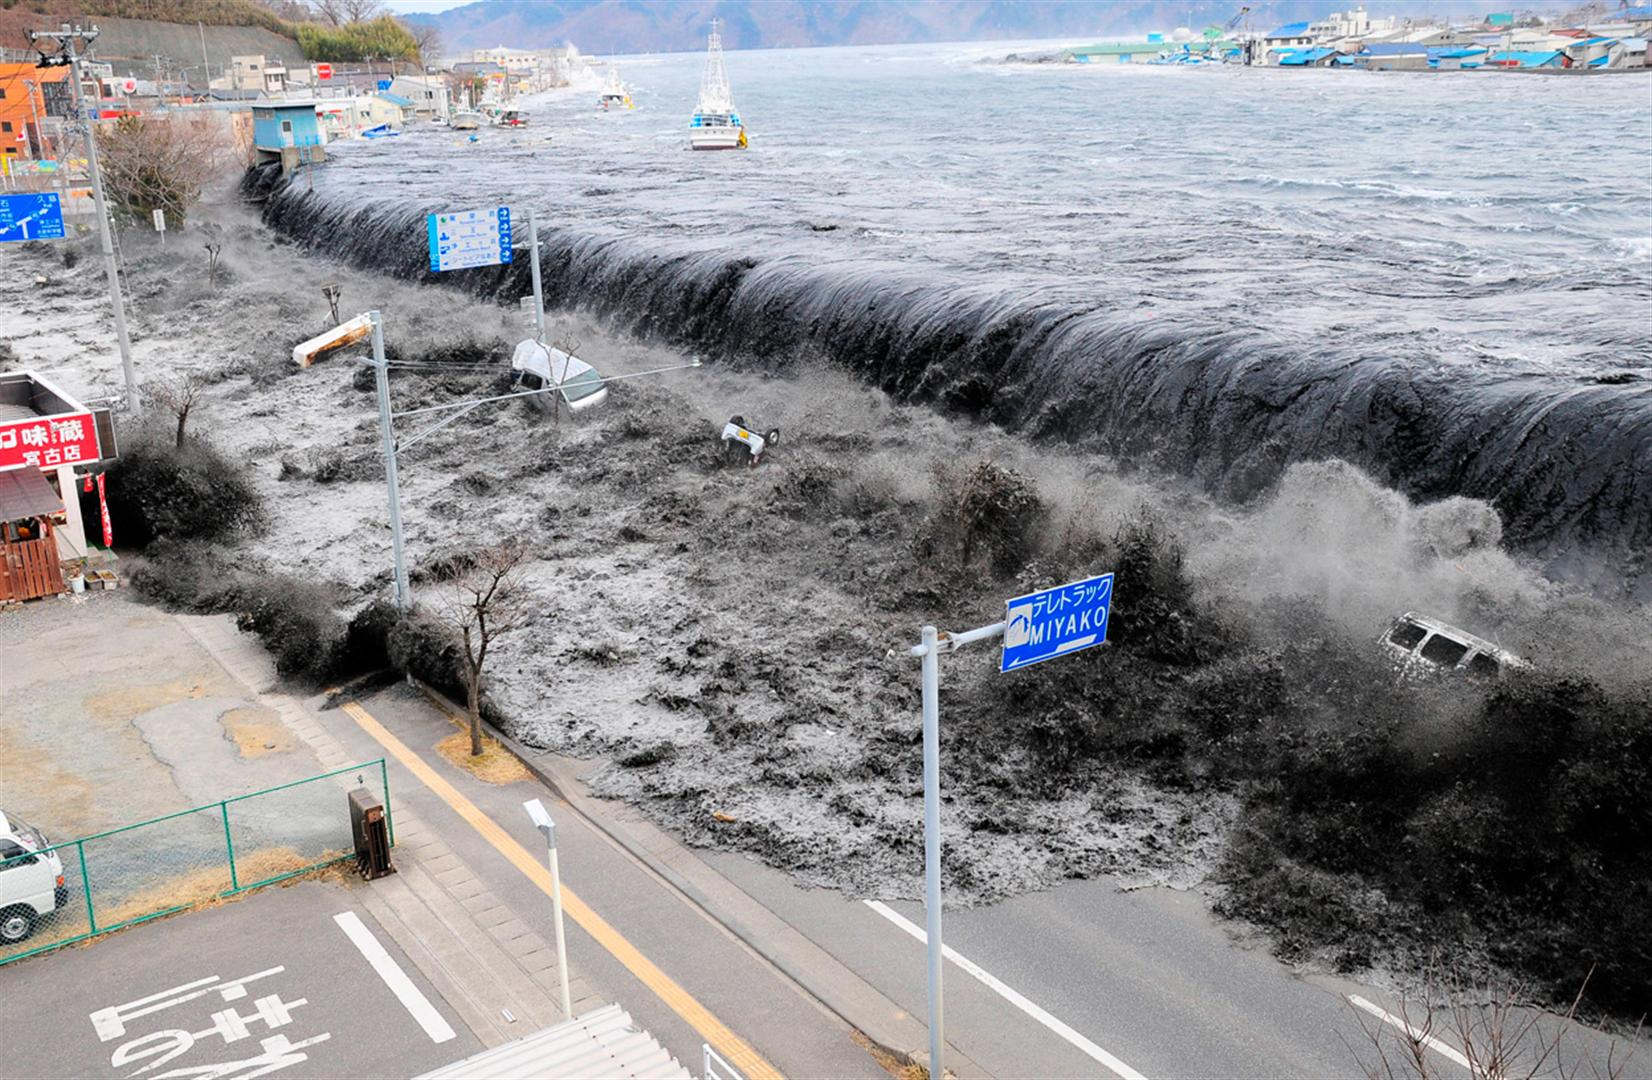
\includegraphics[width=0.42\textwidth,keepaspectratio=true]{tsunami-sendai}

\small tidewater marsh \hfill tsunami inundation

\medskip
\scriptsize and also surface hydrology, subglacial hydrology, \dots
\end{frame}


\section{every time-step is free-boundary problem}

\begin{frame}{semi-discretize in time}

$$h_t + \Div\bq = f \qquad \to \qquad \frac{H_n - H_{n-1}}{\Delta t} + \Div \bQ_n = F_n$$

  \begin{itemize}
  \item semi-discretize in time: $H_n(x) \approx h(t_n,x)$
  \item the new equation is strong form \alert{single time-step problem}
    \begin{itemize}
    \item[$\circ$] a PDE in space where $H_n>0$
    \item[$\circ$] details of flux $\bQ_n$ and source $F_n$ come from time-stepping scheme
      \begin{itemize}
      \item e.g.~$\theta$-methods or RK
      \end{itemize}
    \end{itemize}
  \end{itemize}
\end{frame}


\begin{frame}{weak form incorporates $H_n\ge 0$ constraint}

  \begin{itemize}
  \item define:
    $$\mathcal{K} = \left\{v \in W^{1,p}(\Omega) \,\Big|\, v\ge 0\right\} = \text{\alert{admissible thicknesses}}$$
  \item we say $H_n \in \mathcal{K}$ solves the \alert{weak single time-step problem} if
    $$\int_\Omega H_n (v - H_n) - \Delta t\, \bQ_n \cdot \grad(v - H_n) \ge \int_\Omega \left(H_{n-1} + \Delta t\, F_n\right) (v - H_n)$$
  for all $v \in \mathcal{K}$
  \small
  \medskip
    \begin{itemize}
    \item[$\circ$] derive this \emph{variational inequality} (VI) from:
      \begin{itemize}
      \item[$\diamond$] integration-by-parts on strong form
      \item[$\diamond$] thought about $H_n=0$ areas
      \end{itemize}
    \end{itemize}
  \end{itemize}
\end{frame}


\begin{frame}{weak solves strong but gives more info}

\begin{itemize}
  \item assume $\bQ_n=0$ when $H_n=0$
    \begin{itemize}
    \item[$\circ$] this means $\bQ_n$ describes a \emph{layer}
    \end{itemize}
  \item if $H_n \in \mathcal{K}$ solves weak single time-step problem (VI) then
  
      \medskip
	  \begin{itemize}
	  \item[$\circ$] PDE applies on the set where $H_n>0$ (interior condition):
	    $$\frac{H_n - H_{n-1}}{\Delta t} + \Div \bQ_n = F_n$$
	  \item[$\circ$] plus inequality on the set where $H_n = 0$:
	    $$H_{n-1} + \Delta t\, F_n \le 0$$
	    \vspace{-6mm}
	    \begin{itemize}
	    \item ``climate negative enough during time step to remove old thickness''
	    \end{itemize}
	  \end{itemize}
\end{itemize}
\end{frame}


\begin{frame}{the 3 nonlinearities of the glacier geometry problem}

not counting possible sliding and elevation-accumulation feedbacks
\begin{itemize}
\item the constrained problem (VI or NCP) is inherently nonlinear, i.e.~iteration is needed even for LCPs
\item the $p=n+1$ glen power generates a nonlinearity even in steady state on a flat bed (in that case the ``doubly-nonlinear'' MC equation can be transformed to a straight $p$-laplacian equation)
\item nonzero bedrock gradient ``brings back'' a nonlinearity (Jouvet \& Bueler 2012)
\end{itemize}
\end{frame}


\section{discretization scheme: FVE}

\begin{frame}{finite volume element schemes}

\begin{itemize}
\item FIXME
\end{itemize}

\end{frame}


\begin{frame}{careful: quadrature and upwinding}

\begin{itemize}
\item FIXME
\end{itemize}

\end{frame}


\section{numerical solution: constrained Newton}

\begin{frame}{numerical solution of the weak problem}

the weak single time-step problem:
\begin{itemize}
\item is nonlinear because of constraint (even for $\bQ_n$ linear in $H_n$)
\item can be solved by a Newton method modified for constraint
\item scalable implementations are in PETSc
  \begin{itemize}
  \item[$\circ$]  see ``SNESVI'' object
  \item[$\circ$]  for NCP there are two implementations (Benson \& Munson, 2006):
    \begin{itemize}
    \item  reduced-set (active-set) method
    \item  semismooth method
    \end{itemize}
  \end{itemize}
\end{itemize}

\end{frame}


\section{the essential difficulty} % i.e. bedrock roughness

\begin{frame}{example: Greenland ice sheet}

\begin{columns}
\begin{column}{0.6\textwidth}
\begin{itemize}
\small
\item given steady climate and bedrock elevations, what is shape of Greenland ice sheet?
  \begin{itemize}
  \scriptsize
  \item[$\circ$] climate = ``surface mass balance''
  \item[] \qquad = precipitation $-$ runoff-from-melt
  \end{itemize}
\small
\item assume simplest reasonable dynamics: non-sliding shallow ice approximation
\item solve VI/NCP weak problem
  \begin{itemize}
  \scriptsize
  \item[$\circ$] steady state ($\Delta t\to \infty$)
  \item[$\circ$] reduced-set Newton method
  \item[$\circ$] 900 m structured grid
  \item[$\circ$] $Q^1$ FEs in space
  \item[$\circ$] $N=7\times 10^6$ d.o.f.
  \end{itemize}
\end{itemize}

\vspace{5mm}
\tiny (Bueler, submitted to J.~Glaciol.)
\end{column}
\begin{column}{0.4\textwidth}
\vspace{-5mm}

\begin{center}
\includegraphics[width=0.95\textwidth,keepaspectratio=true]{grnwinset}
\end{center}
\end{column}
\end{columns}
\end{frame}


\begin{frame}{summary}

FIXME consider layer flow model \, $h_t + \Div\bq = f$ \, subject to signed climate $f$ and where $h$ is layer thickness

  \begin{itemize}
  \item goals/issues:
    \begin{itemize}
    \item[$\circ$]  long time steps wanted
    \item[$\circ$]  models have been limited by free-boundary lack-of-clarity
    \end{itemize}
  \item approach:
    \begin{itemize}
    \item[$\circ$]  include constraint on thickness: $h\ge 0$
    \item[$\circ$]  consider discrete-time problem before doing FEM/FVM/etc.
    \item[$\circ$]  pose single time-step problem weakly as VI or NCP
    \item[$\circ$]  solve by scalable constrained-Newton method (PETSc)
    \end{itemize}
  \end{itemize}

\end{frame}

\end{document}
